\documentclass[11pt]{scrartcl}
\usepackage[sexy]{{style_files/evan}}

\usepackage{{style_files/NMC}}
\usepackage{standalone}
\usepackage{import}

\usepackage{tkz-euclide} % For usage in NMC8G1

\begin{document}
\title{NMC Problem Set \#8} % add # of pset
\date{Oct. 9, 2022} % add date
\maketitle

\section*{Welcome!}

This is a selection of interesting problems derived from curious thoughts, curated so you can nibble on them throughout the week! The point of this document is to introduce you to fun puzzles that require thinking. We recommend you try the ones that you find interesting! Feel free to work on them with others (even us teachers!). Harder problems are marked with chilies (\fullchili), in case you want to challenge yourself.
\newline\newline
Have fun! \textit{Note: New variants on these problems may be released throughout the week. Remember to check back once in a while!}
    
\section{Algebra}
\begin{enumerate}[label=\textbf{A\arabic*}.]
    \item (\fullchili) \textbf{Searching for a Simplification} \newline
    Determine all integers $n$ such that
    \[ x_1^2 + x_2^2 + x_3^2 + \dots + x_n^2 \geq n\sum_{\mathrm{cyc}} \left( x_i x_{i+1} \right) \]
    for any choice of non-negative real sequences $(x_n)$.
    
    \item \textbf{Three positive roots} \newline
    The polynomial $x^3 + ax^2 + bx + c$ has three positive roots. Prove that $27c \geq a^3$ and $a^2 \geq 3b$.
\end{enumerate}

\newpage
\section{Combinatorics}
\begin{enumerate}[label=\textbf{C\arabic*}.]
    \item \textbf{Monty Hall's Game Show} \newline
    You are in a game show, asked to choose between a set of $n$ doors. Behind each door is either a car or a goat ($1$ car and $n-1$ goats). First, you pick a door. Then, the host, Monty Hall, picks another door, different from the one you picked (and by the game show's rules, he opens a door with a goat behind it).
    
    \begin{theorem}[Bayes' Theorem]
        This problem uses the concept of \textbf{conditional probability}, defined as follows:
        \[ P(A \mid B) = \frac{P(A \cap B)}{P(B)}. \]
        This reads as: "the probability of event $A$ occurring given that $B$ occurs is equal to the probability of \textit{both} $A$ and $B$ occurring divided by the probability of $B$ occurring." From this, we can deduce Bayes' Formula:
        \[ P(A \mid B) = \frac{P(B \mid A) \cdot P(A)}{P(B)}. \]
    \end{theorem}
    
    \begin{enumerate}
        \item In the classic Monty Hall problem, we have $n = 3$ doors. After Monty Hall reveals a door containing a goat and assuming you prefer cars over goats, should you switch your choice?
        
        \item Suppose that Monty Hall has forgotten where the car and the goats are! He still opens a door, but this time, he just \textit{happens} to reveal a goat instead of a car. Assuming that you still prefer cars over goats, is it reasonable to switch your initial door of choice?
        
        \item (\halfchili) Suppose now that we have $n$ doors and Monty Hall decides to reveal $0 \leq k \leq n-1$ of them, showing only goats. For which values of $k$ should you switch your choice of door? What's your best chance at winning a car for any given $n, k$?
        
        \item (\halfchili) Let's say that $3$ people are playing in the Monty Hall Game Show with $n = 3$ doors. Monty assigns a (different) door to each of the $3$ contestants, and picks one person who, unfortunately, was given a goat door, and instructs him to open it. The contestant walks away with a goat. The last two people are now faced with a choice: is it better for them to switch, or to keep the door that they have... or is there something amiss here?
    \end{enumerate}
    
    \begin{figure}[h]
        \centering
        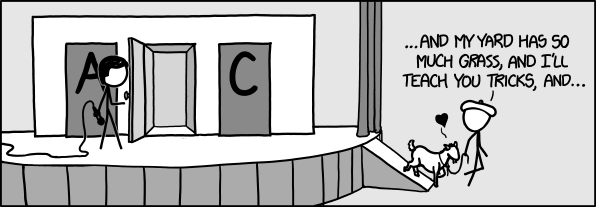
\includegraphics[width = 11cm]{Diagrams/Monty Hall.png}
        \caption{Source: \href{https://xkcd.com/1282/}{Thanks, XKCD!}}
        \label{fig:Monty_Hall}
    \end{figure}
    
\end{enumerate}

\newpage
\section{Geometry}
\begin{enumerate}[label=\textbf{G\arabic*}.]
  \item \textbf{Maximizing the perimeter on an Ark(yter)} \newline
  Let points $A$ and $B$ be given on a circle $\Gamma$. Let a point $C$ vary on one of the arcs $AB$ of $\Gamma$. Prove that the perimeter of triangle $\triangle ABC$ is maximized when $C$ is the midpoint of this arc.
  
    \begin{figure}[h]
        \centering
        \includegraphics[width = 8cm]{Diagrams/Week 8 Maximizing Perimeter.tex}
    \end{figure}
\end{enumerate}

\newpage
\section{Number Theory}
\begin{enumerate}[label=\textbf{N\arabic*}.]
    \item \textbf{LCM and GCD!} \newline
    The LCM (Lowest Common Multiple) and GCD (Greatest Common Divisor) are two important number theoretic functions! Here are some problems.
    
    \begin{enumerate}
        \item First, show that
        \[ \gcd(p, q) \cdot \lcm(p, q) = pq. \]
    
        \item (\halfchili) Suppose that $p < q$ are positive integers with
        \[ \gcd(p, q) + \lcm(p, q) = p + q. \]
        Show that $p$ divides into $q$.
        
        \item (\fullchili) Let $m \geq 2$ be a positive integer and $a, b \in \ZZ^+$. Prove \[ \gcd(m^a - 1, m^b - 1) = m^{\gcd(a, b)} - 1. \]
        
        \item (\fullchili) Let $a, b, c$ be positive integers. If
        \[ \gcd(a, b, c) \cdot \lcm(a, b, c) = abc, \]
        prove that $\gcd(a, b) = \gcd(b, c) = \gcd(a, c) = 1$.
    \end{enumerate}
    
    \item (\fullchili \hspace{1pt} $\times$ 1.5) \textbf{The Erd\H{o}s-Suranyi Problem} \newline
    Prove that every number $n$ can be written in the following form,
    \[ n = \pm 1^2 \pm 2^2 \pm 3^2 \pm 4^2 \pm 5^2 \pm \dots. \]
\end{enumerate}
\end{document}
